\documentclass{article}
\usepackage{graphicx}
\usepackage{geometry}
\usepackage{hyperref}
\usepackage{booktabs}
\usepackage{amsmath}
\usepackage{amssymb}
\usepackage{longtable}
\usepackage{xcolor}

\geometry{a4paper, margin=0.8in}

\hypersetup{colorlinks=true, linkcolor=blue, urlcolor=cyan}

\title{Gradient-Geometry Baselines ($f=0$) and Their Correlation\\with Robustness Under Attack}
\author{ByzFL SNN Benchmark}
\date{\today}

\begin{document}
\maketitle

\tableofcontents
\newpage

\section{Setup}

\subsection{Gradient-geometry baselines}
Three models are trained on MNIST with $n=10$ honest clients, $f=0$ (no Byzantine clients, \texttt{NoAttack}), aggregator \texttt{TrMean} with pre-aggregators \texttt{NNM}+\texttt{ARC}, across four data-heterogeneity levels $\gamma \in \{1.0, 0.66, 0.33, 0.0\}$ (\texttt{gamma\_similarity\_niid}), for 500 training steps, 1 seed:
\begin{itemize}
    \item \textbf{SNN (atan, $\alpha=1.2$)}: \texttt{cnn\_mnist\_snn}, LIF layers, surrogate gradient \texttt{atan}, $\beta=0.95$, threshold $=1.0$, $T=10$ time steps, lr $=0.10$.
    \item \textbf{CNN ReLU}: \texttt{cnn\_mnist}, lr $=0.15$.
    \item \textbf{CNN Tanh}: \texttt{cnn\_mnist\_tanh}, lr $=0.15$.
\end{itemize}
All three models have $d = 431{,}080$ parameters (identical architecture, only the activation/neuron model differs). Metrics are computed online, every training step, directly on the honest, post-momentum gradient vectors actually used for aggregation --- no raw vectors are ever logged to disk.

\subsection{Robustness sources (existing sweeps)}
\label{sec:robustness-sources}
These robustness sweeps were originally run on a separate Docker host; only a \emph{subset} of the full grid was imported into this local repository, not the complete sweep output. As a result, no locally-available sweep matches all of the geometry baseline's hyperparameters (aggregator, learning rate, SNN $\alpha$) with complete $f\in\{0,\dots,5\}$, $\gamma$, and attack coverage --- only whatever combination of (aggregator, lr/$\alpha$, attack) happened to be imported is usable here. The best available \emph{common} aggregator with full $(f,\gamma,\text{attack})$ coverage for all three models among the imported data is \texttt{GeometricMedian}+\texttt{NNM}+\texttt{ARC} (not \texttt{TrMean}, which is only fully covered for CNN~Tanh). The sources actually used:

\begin{center}
\begin{tabular}{@{}lll@{}}
\toprule
Model & Results directory & Deviation from geometry baseline \\
\midrule
SNN atan & \texttt{results/snn/robust\_new\_atan\_sweep} & $\alpha=1.25$ (only $\alpha\in\{0.5,0.75,1.0,$ \\
 & & $1.25,1.5,2.0,3.0\}$ were imported, not 1.2; \\
 & & 1.25 is the closest); only \texttt{Optimal\_ALittleIsEnough\_neg1} \\
 & & was imported for this combo (single-attack, not worst-of-3) \\
CNN ReLU & \texttt{results/cnn/weekend} & lr$=0.05$ (the lr$=0.15$ import, \\
 & & \texttt{robust\_comparison\_sweep}, only covers $f=0..2$); \\
 & & worst-of-3 attacks \\
CNN Tanh & \texttt{results/cnn/tanh\_heatmap\_sweep} & lr$=0.15$, exact match; worst-of-3 attacks \\
\bottomrule
\end{tabular}
\end{center}

For each $(f,\gamma)$ cell, the accuracy score is the mean test accuracy over the last three evaluation checkpoints (steps 400, 450, 500), averaged over 5 training seeds, then the \emph{worst case over available attacks} (minimum), matching the convention already used by the repository's own \texttt{test\_heatmap} utility. This substitution of aggregator/lr/$\alpha$ means the robustness numbers below are a \emph{proxy}, not an exact match to the geometry-baseline training dynamics; the geometry metrics themselves come only from the exact-match $f=0$/\texttt{TrMean} runs described above.

\section{Metric Definitions}

Let $\{m^{(k)}\}_{k=1}^{n}$ be the honest, post-momentum gradient vectors at a given training step ($n=10$). For each coordinate $j$:
\begin{align}
\mu_j &= \frac{1}{n}\sum_{k=1}^n m^{(k)}_j
& \sigma_j &= \sqrt{\frac{1}{n}\sum_{k=1}^n \left(m^{(k)}_j - \mu_j\right)^2} \\
\text{CV}_j &= \frac{\sigma_j}{|\mu_j| + 10^{-12}}
& A_j &= \frac{\max\!\big(\#\{k: m^{(k)}_j > 0\},\ \#\{k: m^{(k)}_j < 0\}\big)}{n}
\end{align}
where $|m^{(k)}_j| < 10^{-12}$ abstains from the sign count in $A_j$ (denominator $n$ stays fixed).

\textbf{Scalar summaries} (one value per training step):
\begin{align}
N &= \frac{\text{std}_k\big(\lVert m^{(k)} \rVert_2\big)}{\text{mean}_k\big(\lVert m^{(k)} \rVert_2\big) + 10^{-12}}
&& \text{(dispersion of per-client gradient norms)} \\
Q &= \frac{1}{d}\sum_{j=1}^d \mathbb{1}[A_j \ge 0.8]
&& \text{(raw fraction of coordinates in sign-consensus)} \\
S &= \frac{\sum_j \mu_j^2 \cdot \mathbb{1}[A_j \ge 0.8]}{\sum_j \mu_j^2 + 10^{-12}}
&& \text{(signal-weighted consensus)} \\
\cos_{\text{mean}} &= \underset{k < l}{\text{mean}}\ \frac{\langle m^{(k)}, m^{(l)}\rangle}{\lVert m^{(k)}\rVert \lVert m^{(l)}\rVert}
&& \text{(mean pairwise cosine similarity)}
\end{align}

\textbf{Per-layer breakdown}: for a layer $L$ spanning coordinate range $[a_L, b_L)$, $Q_L$ and $S_L$ are computed identically but restricted to that range. $S_{\text{layer0}}$ denotes the first weight-bearing layer (\texttt{conv1} for the SNN, \texttt{\_c1} for the CNNs); $S_{\text{deep\_mean}}$ is the mean of $S_L$ over all other layers.

\textbf{Summary statistic used below}: for each (model, $\gamma$) run, we take the \emph{median} of each per-step metric over steps $\in [100, 400]$ (the ``established regime'' window, chosen after visually inspecting the trajectories -- see Section~\ref{sec:trajectories}).

\section{Geometry Trajectories}
\label{sec:trajectories}

\begin{figure}[htbp]
    \centering
    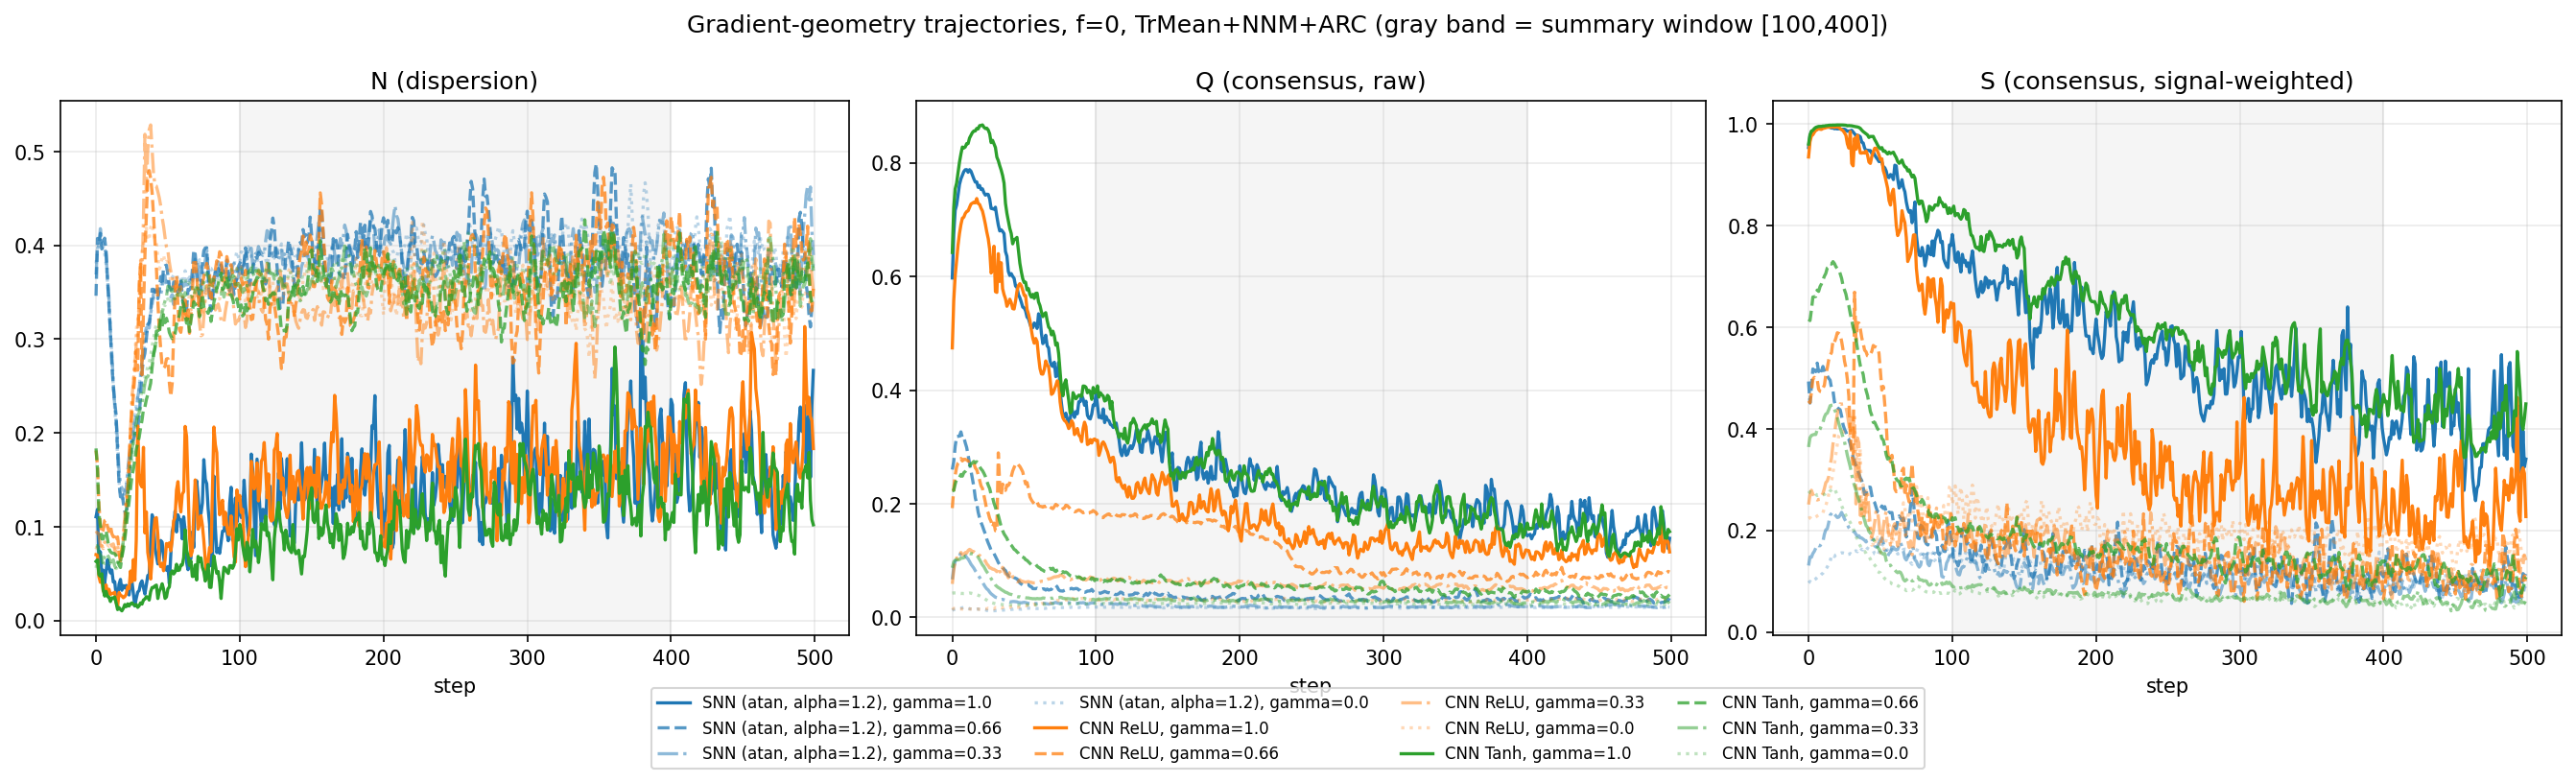
\includegraphics[width=\textwidth]{trajectories_N_Q_S.png}
    \caption{$N(\tau)$, $Q(\tau)$, $S(\tau)$ over training, one curve per (model, $\gamma$). Solid = $\gamma=1.0$, dashed = $0.66$, dash-dot = $0.33$, dotted = $0.0$. Blue = SNN, orange = CNN ReLU, green = CNN Tanh. Gray band marks the [100,400] summary window.}
    \label{fig:trajectories}
\end{figure}

\textbf{Observed fact}: at $\gamma=1.0$ (solid curves), $S$ keeps decreasing slowly through the entire [100,400] window rather than reaching a stable plateau; at $\gamma<1.0$, all three models reach a noisy plateau by step $\sim$150. The [100,400] median is therefore a ``passing value'' rather than a true steady state for the $\gamma=1.0$ runs.

\subsection{Trajectories split by $\gamma$ (direct 3-model comparison)}
The figure above overlays all 12 (model, $\gamma$) curves per panel, which makes it hard to compare the 3 models at a fixed $\gamma$. Figures~\ref{fig:traj-gamma-10}--\ref{fig:traj-gamma-00} below show the same $N(\tau)$, $Q(\tau)$, $S(\tau)$ data, one figure per $\gamma$, with only the 3 models overlaid (blue = SNN, orange = CNN ReLU, green = CNN Tanh).

\begin{figure}[htbp]
    \centering
    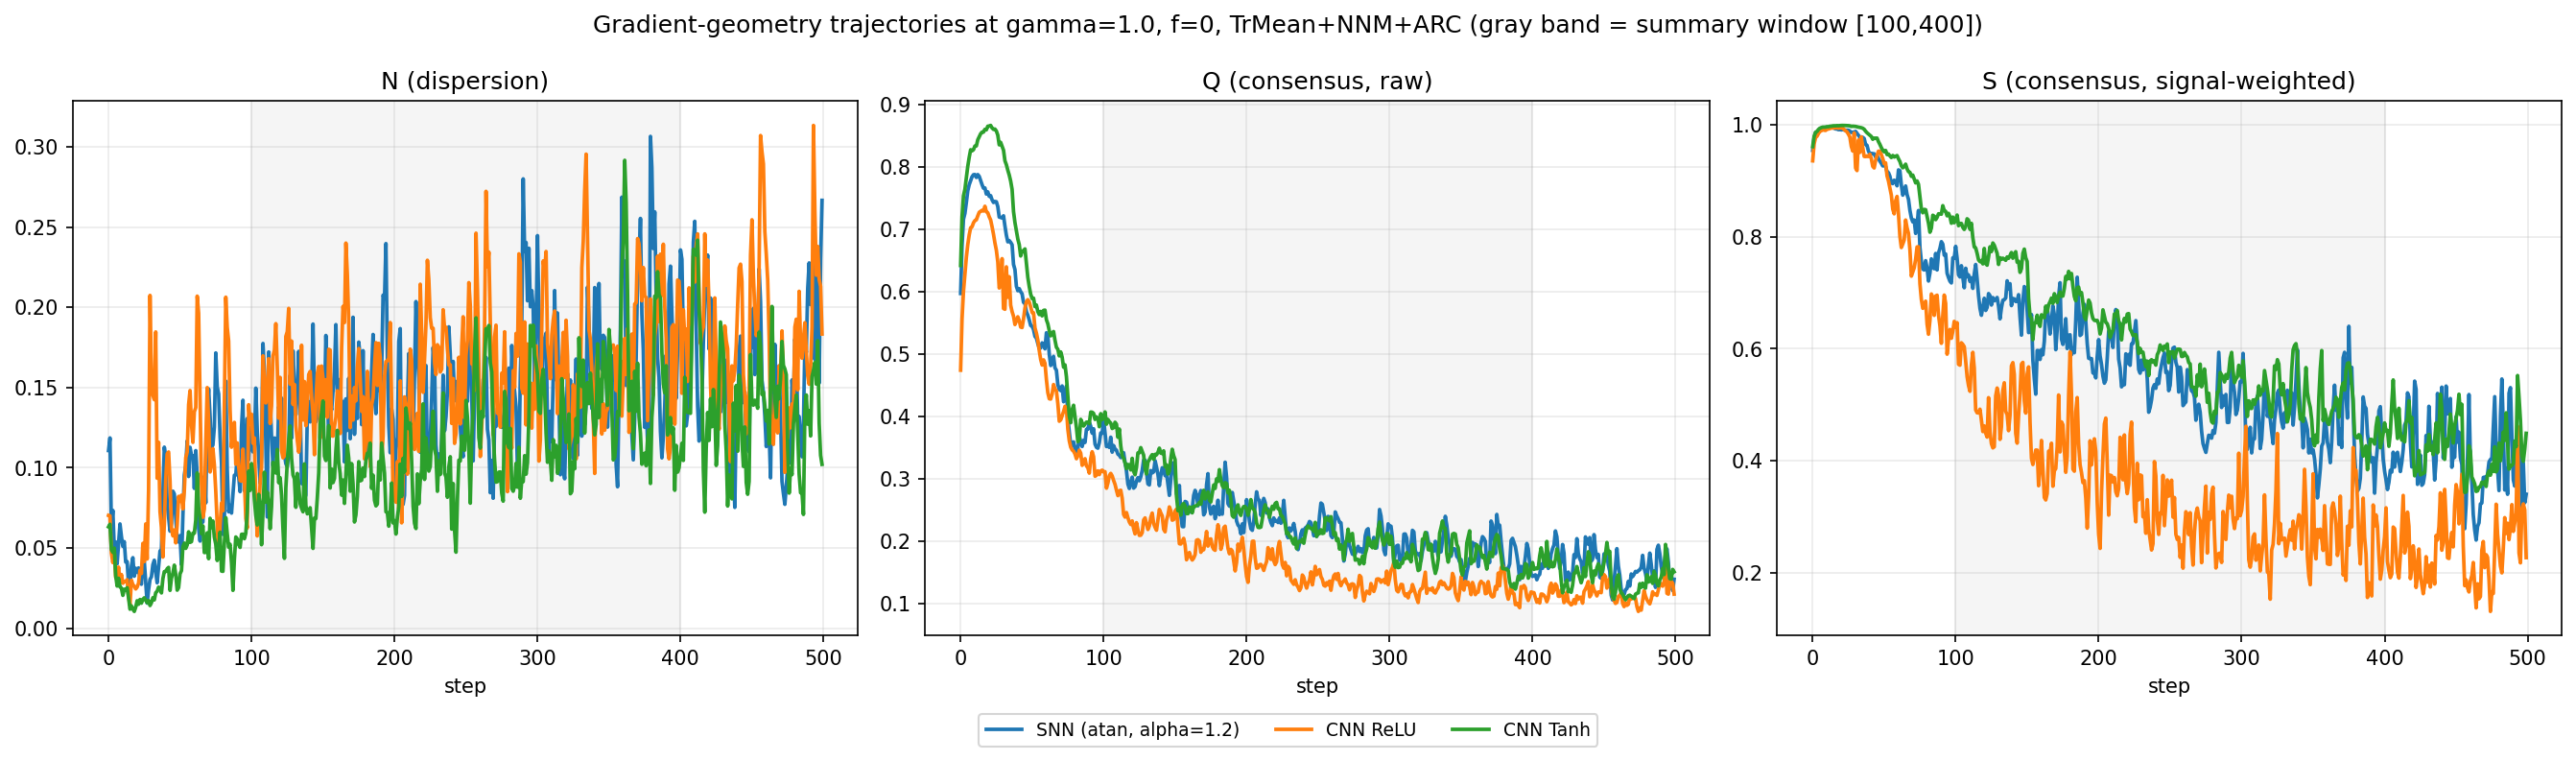
\includegraphics[width=\textwidth]{trajectories_gamma_10.png}
    \caption{$\gamma=1.0$: the 3 models compared directly.}
    \label{fig:traj-gamma-10}
\end{figure}

\begin{figure}[htbp]
    \centering
    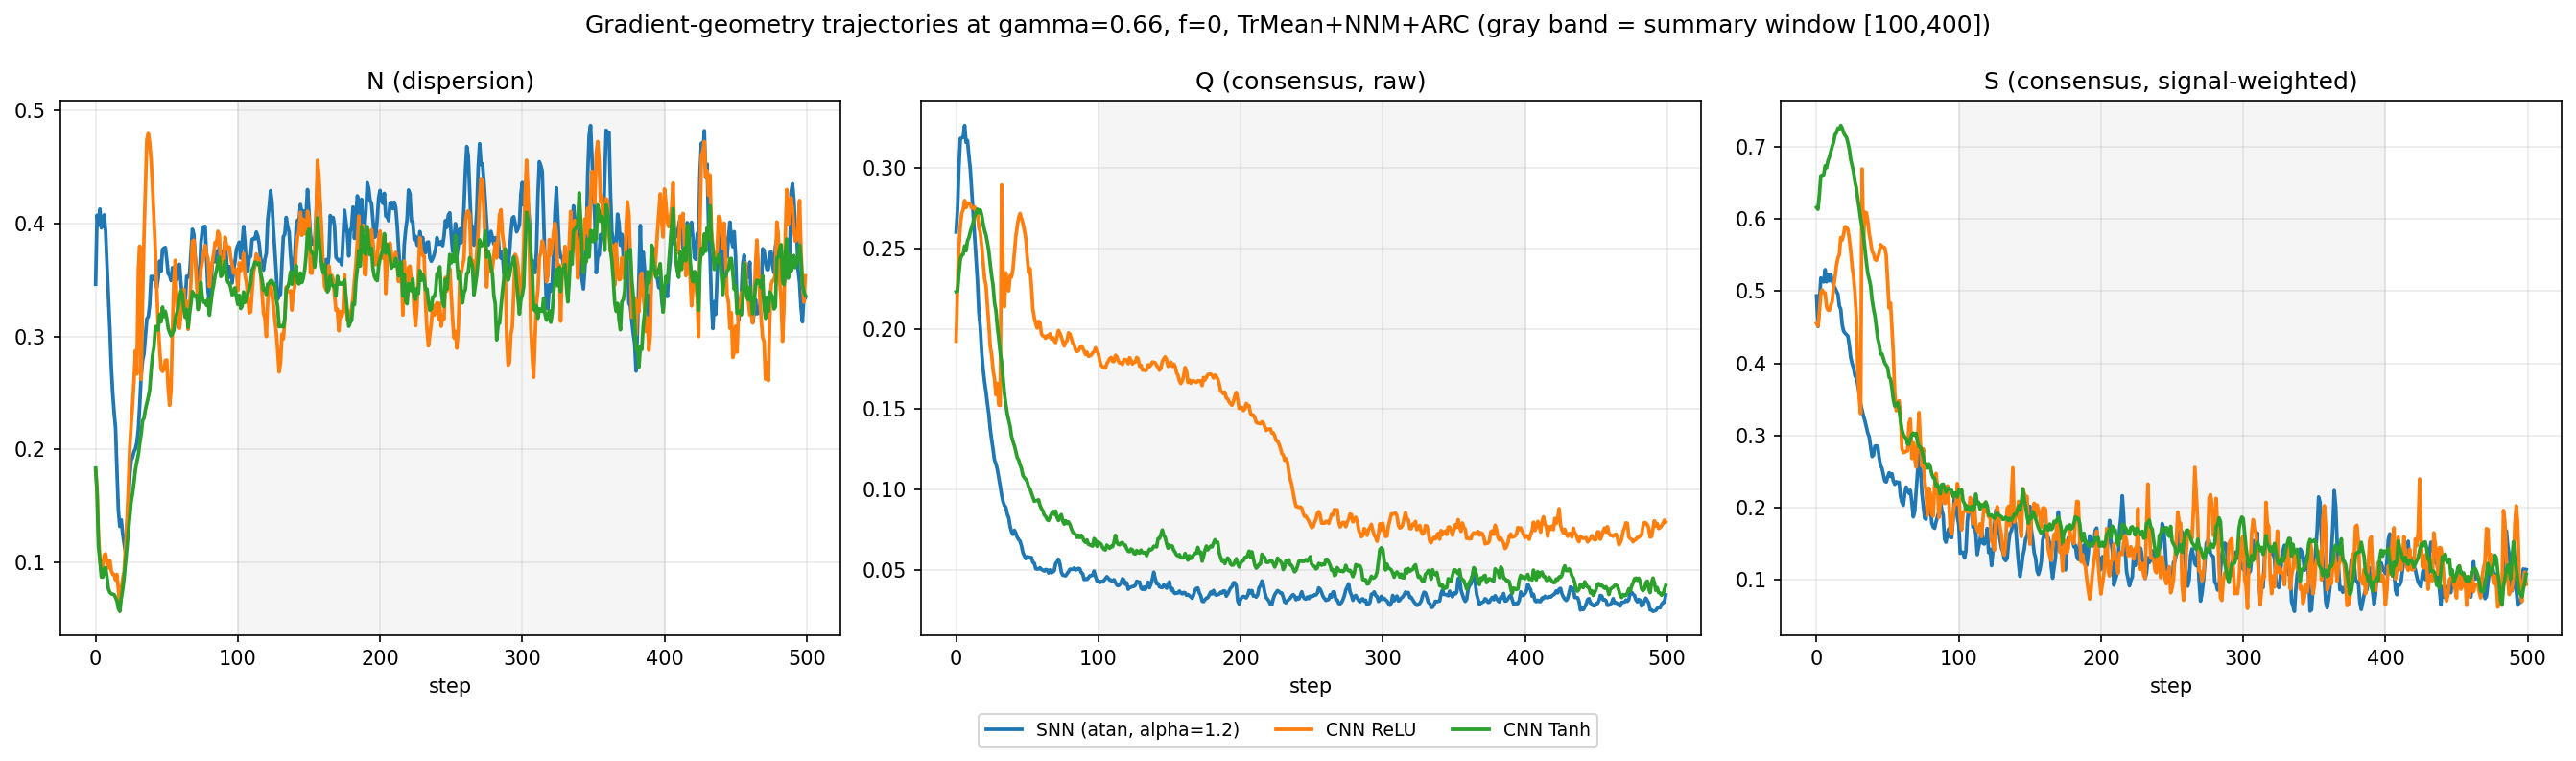
\includegraphics[width=\textwidth]{trajectories_gamma_066.png}
    \caption{$\gamma=0.66$: the 3 models compared directly.}
    \label{fig:traj-gamma-066}
\end{figure}

\begin{figure}[htbp]
    \centering
    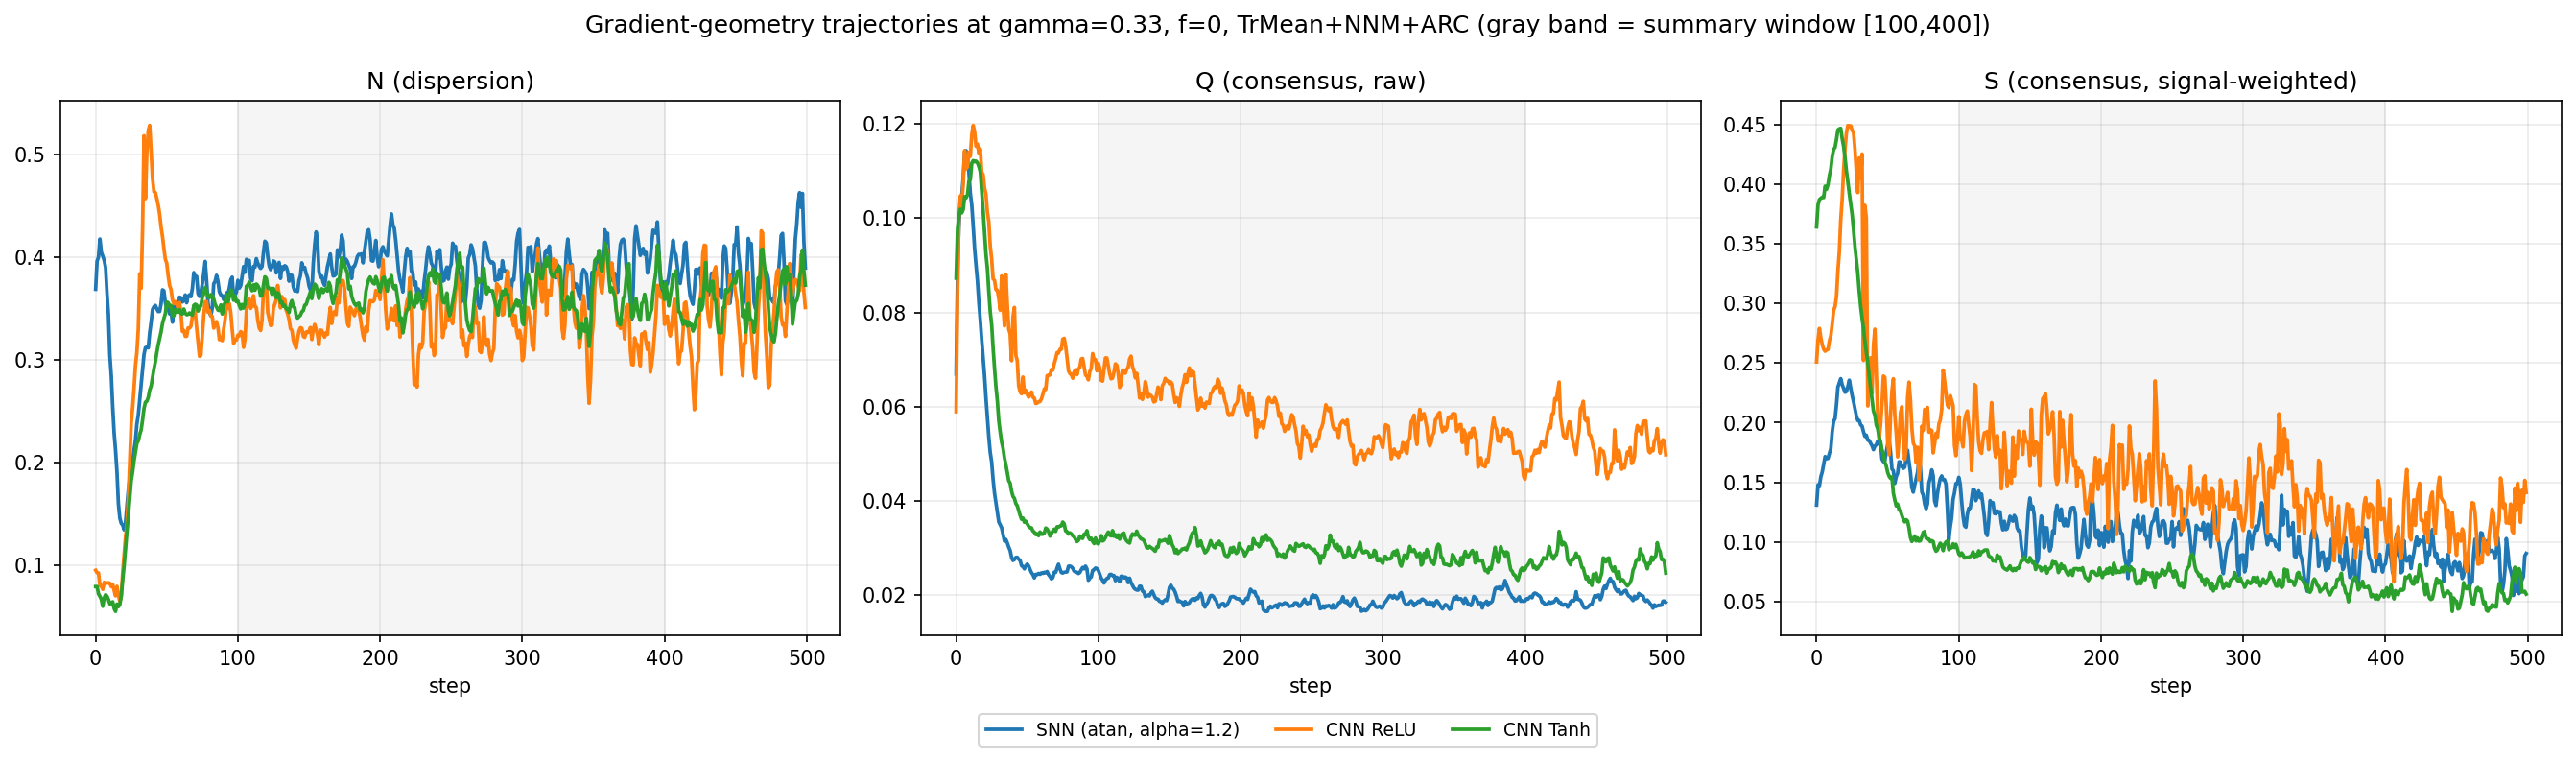
\includegraphics[width=\textwidth]{trajectories_gamma_033.png}
    \caption{$\gamma=0.33$: the 3 models compared directly.}
    \label{fig:traj-gamma-033}
\end{figure}

\begin{figure}[htbp]
    \centering
    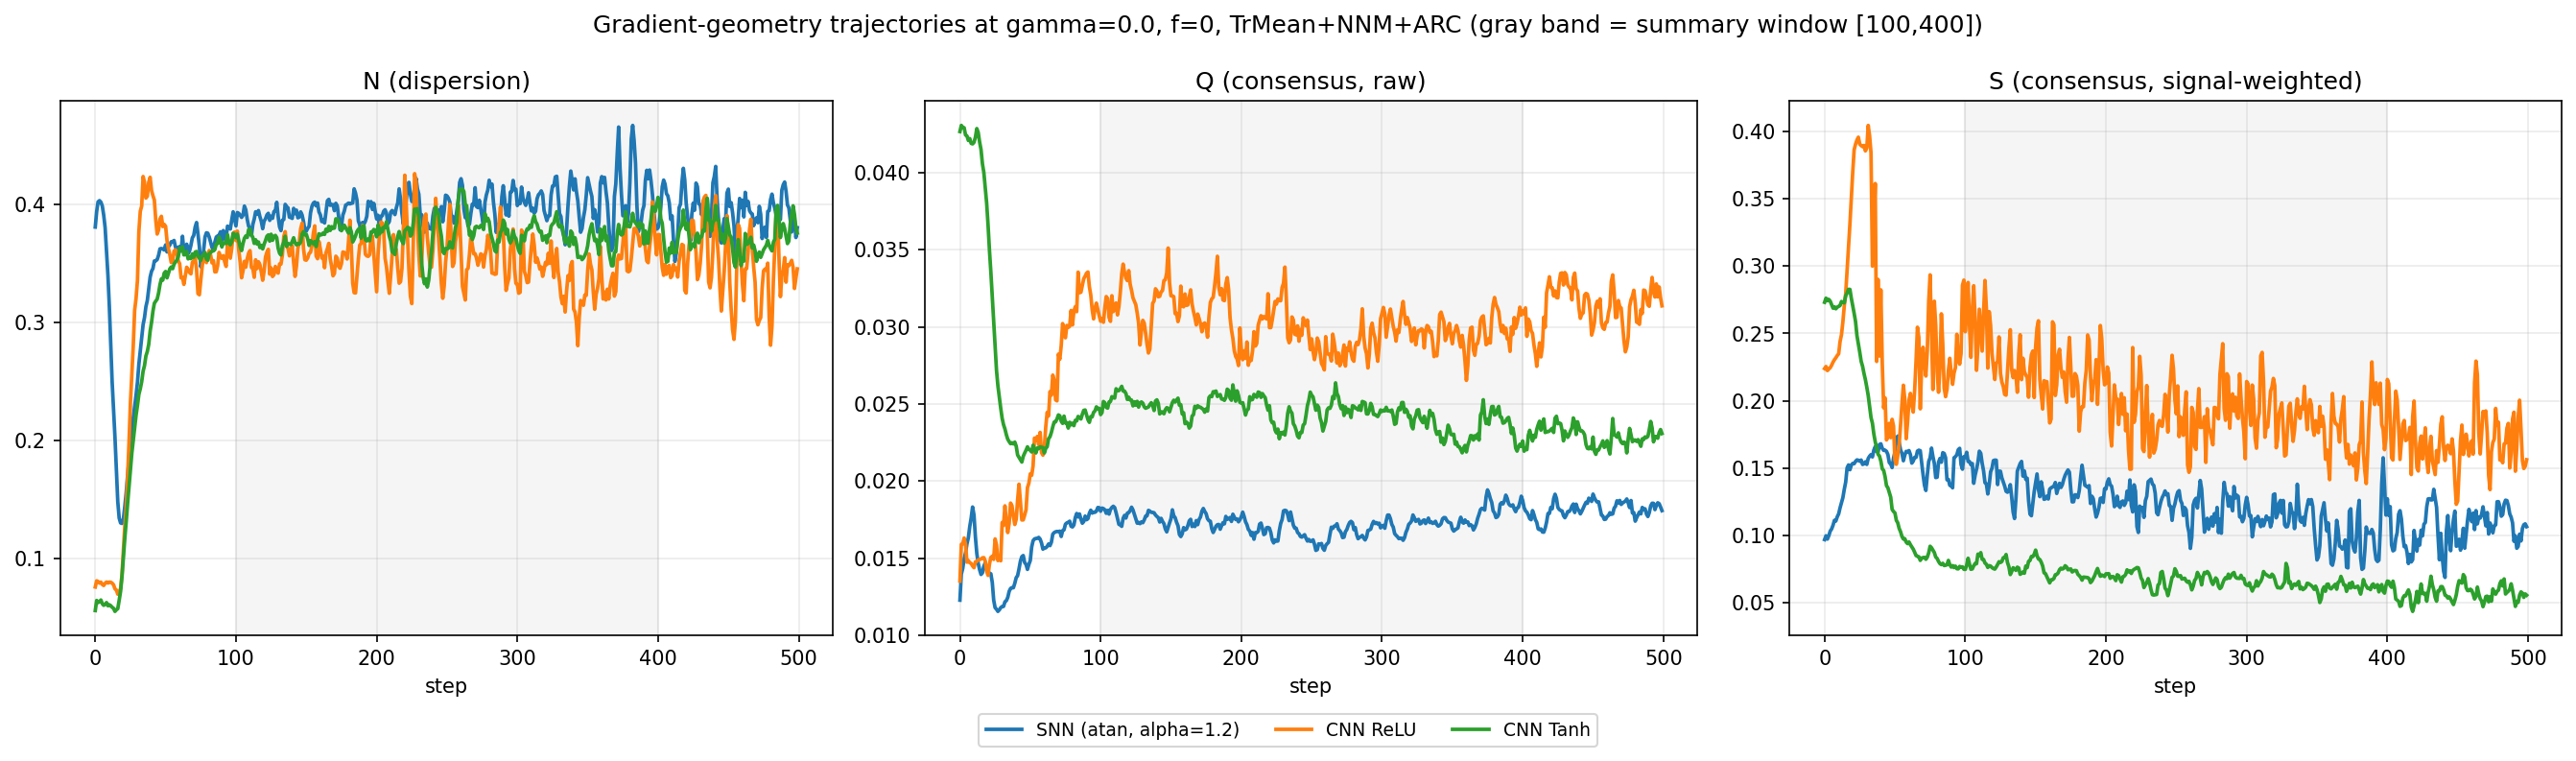
\includegraphics[width=\textwidth]{trajectories_gamma_00.png}
    \caption{$\gamma=0.0$: the 3 models compared directly.}
    \label{fig:traj-gamma-00}
\end{figure}

\clearpage
\section{Geometry Summary Table}

\begin{center}
\small
\begin{tabular}{@{}llrrrrr@{}}
\toprule
Model & $\gamma$ & $N$ & $Q$ & $S$ & $S_{\text{layer0}}$ & $\cos_{\text{mean}}$ \\
\midrule
SNN atan     & 1.0  & 0.143 & 0.223 & 0.547 & 0.624 & 0.085 \\
SNN atan     & 0.66 & 0.388 & 0.034 & 0.132 & 0.161 & $-0.074$ \\
SNN atan     & 0.33 & 0.391 & 0.019 & 0.108 & 0.055 & $-0.086$ \\
SNN atan     & 0.0  & 0.395 & 0.017 & 0.124 & 0.048 & $-0.087$ \\
\addlinespace
CNN ReLU     & 1.0  & 0.158 & 0.143 & 0.331 & 0.648 & 0.004 \\
CNN ReLU     & 0.66 & 0.362 & 0.085 & 0.137 & 0.069 & $-0.082$ \\
CNN ReLU     & 0.33 & 0.341 & 0.057 & 0.150 & 0.018 & $-0.093$ \\
CNN ReLU     & 0.0  & 0.354 & 0.030 & 0.198 & 0.012 & $-0.093$ \\
\addlinespace
CNN Tanh     & 1.0  & 0.106 & 0.216 & 0.591 & 0.552 & 0.107 \\
CNN Tanh     & 0.66 & 0.352 & 0.053 & 0.155 & 0.145 & $-0.071$ \\
CNN Tanh     & 0.33 & 0.365 & 0.029 & 0.072 & 0.025 & $-0.090$ \\
CNN Tanh     & 0.0  & 0.374 & 0.025 & 0.068 & 0.014 & $-0.092$ \\
\bottomrule
\end{tabular}
\end{center}
Median over steps $\in[100,400]$. Full table with q25/q75 in \texttt{summary\_table.csv}.

\subsection{Registered predictions, checked against these numbers}
\begin{center}
\small
\begin{tabular}{@{}lp{9cm}@{}}
\toprule
Prediction & Verdict \\
\midrule
$S_{\text{SNN}} < S_{\text{ReLU}}$ and $S_{\text{SNN}} < S_{\text{Tanh}}$ at every $\gamma$ & Holds only at $\gamma=0.66$. At $\gamma=1.0$, $S_{\text{ReLU}}=0.331$ is the \emph{lowest} of the three, not the SNN ($0.547$). \\
$N_{\text{ReLU}} \gg N_{\text{SNN}} \approx N_{\text{Tanh}}$ & Violated at 3 of 4 $\gamma$ values; only $\gamma=1.0$ confirms it. Elsewhere all three models have near-identical $N$ (see Section~\ref{sec:trajectories}: $N$ clusters by $\gamma$, not by model). \\
$S$ decreases monotonically as $\gamma$ decreases, for all models & Holds only for CNN Tanh. SNN and ReLU both tick up slightly between $\gamma=0.33$ and $\gamma=0.0$. \\
$S_{\text{layer0}}(\text{SNN}) \gg S_{\text{deep\_mean}}(\text{SNN})$ & Holds only at $\gamma=1.0$ (0.624 vs.\ 0.579, small margin). At $\gamma<1.0$ the deep layers have \emph{higher} consensus than layer0, with the gap widening as $\gamma\to 0$. \\
\bottomrule
\end{tabular}
\end{center}

\section{Robustness Heatmaps}

\begin{figure}[htbp]
    \centering
    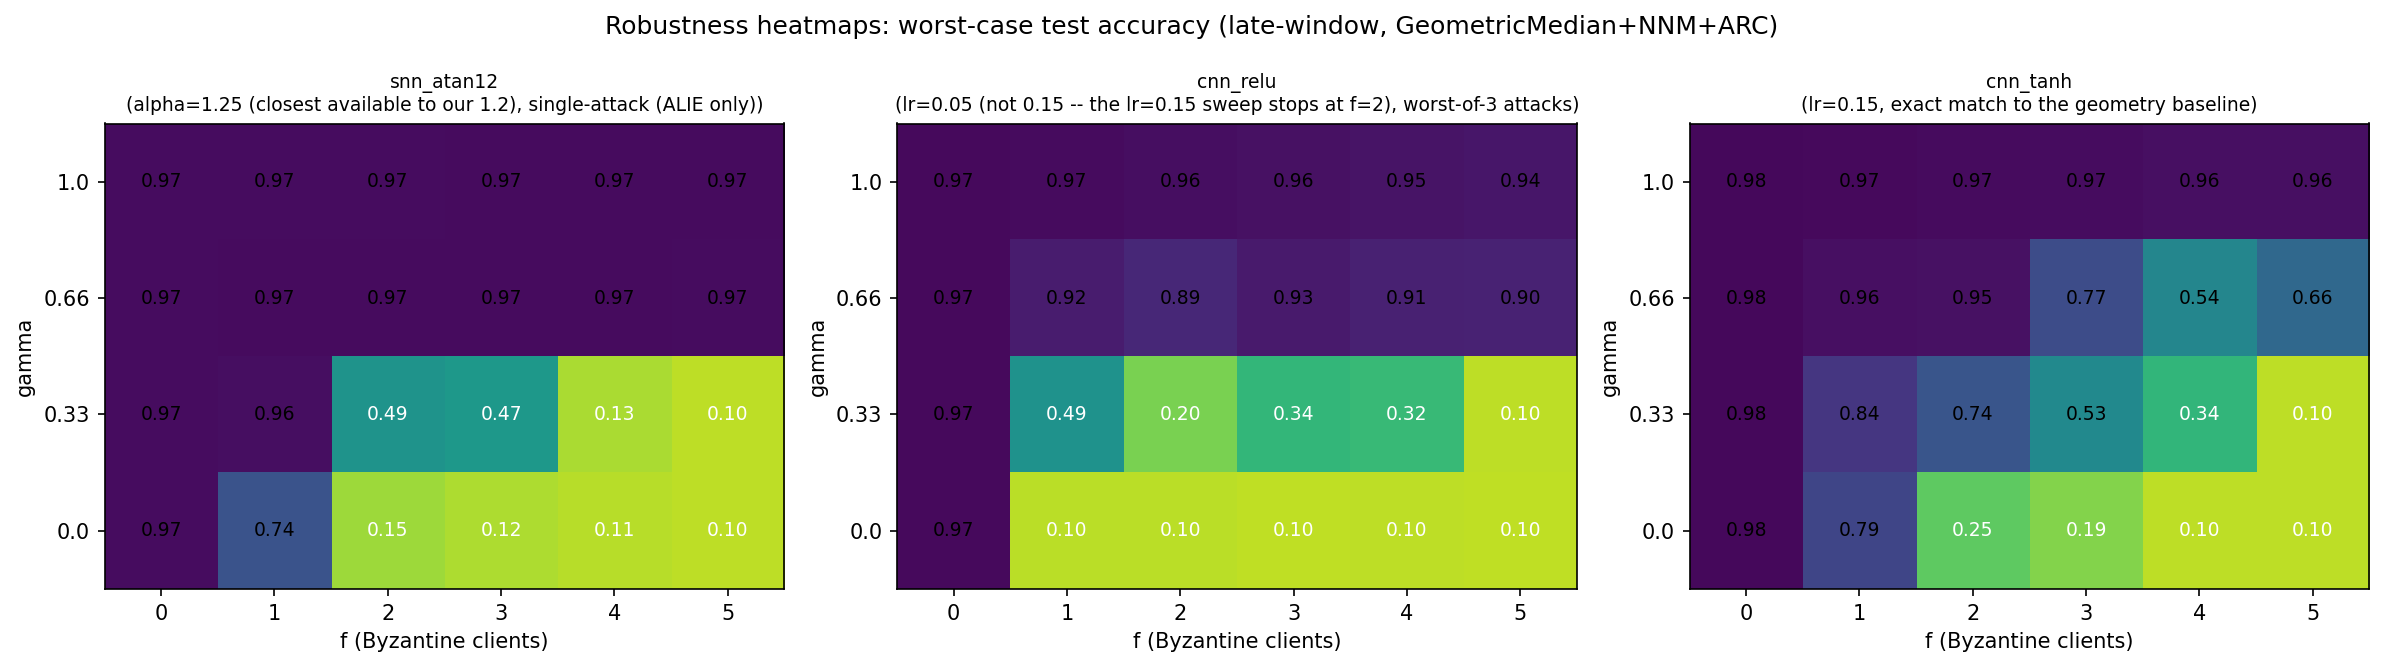
\includegraphics[width=\textwidth]{robustness_heatmaps.png}
    \caption{Worst-case (min-over-attacks) test accuracy, late-window average, per (model, $f$, $\gamma$). Aggregator \texttt{GeometricMedian}+\texttt{NNM}+\texttt{ARC}. See Section~\ref{sec:robustness-sources} for the exact hyperparameter deviations per model.}
    \label{fig:robustness-heatmaps}
\end{figure}

\textbf{Observed facts}: all three models are near-perfectly robust at $\gamma=1.0$ across every $f$ tested (accuracy stays $\ge 0.94$). At $\gamma \le 0.66$, accuracy collapses toward $\sim$0.10 (chance level on 10 classes) once $f \ge 2$--$3$, for all three models. CNN~Tanh degrades more gradually at $\gamma=0.66$ (e.g.\ $0.96 \to 0.54$ across $f=0..4$) than SNN or CNN~ReLU, which drop sharply.

\section{Correlation: Geometry ($f=0$) vs.\ Robustness (attacked, $f>0$)}

\begin{figure}[htbp]
    \centering
    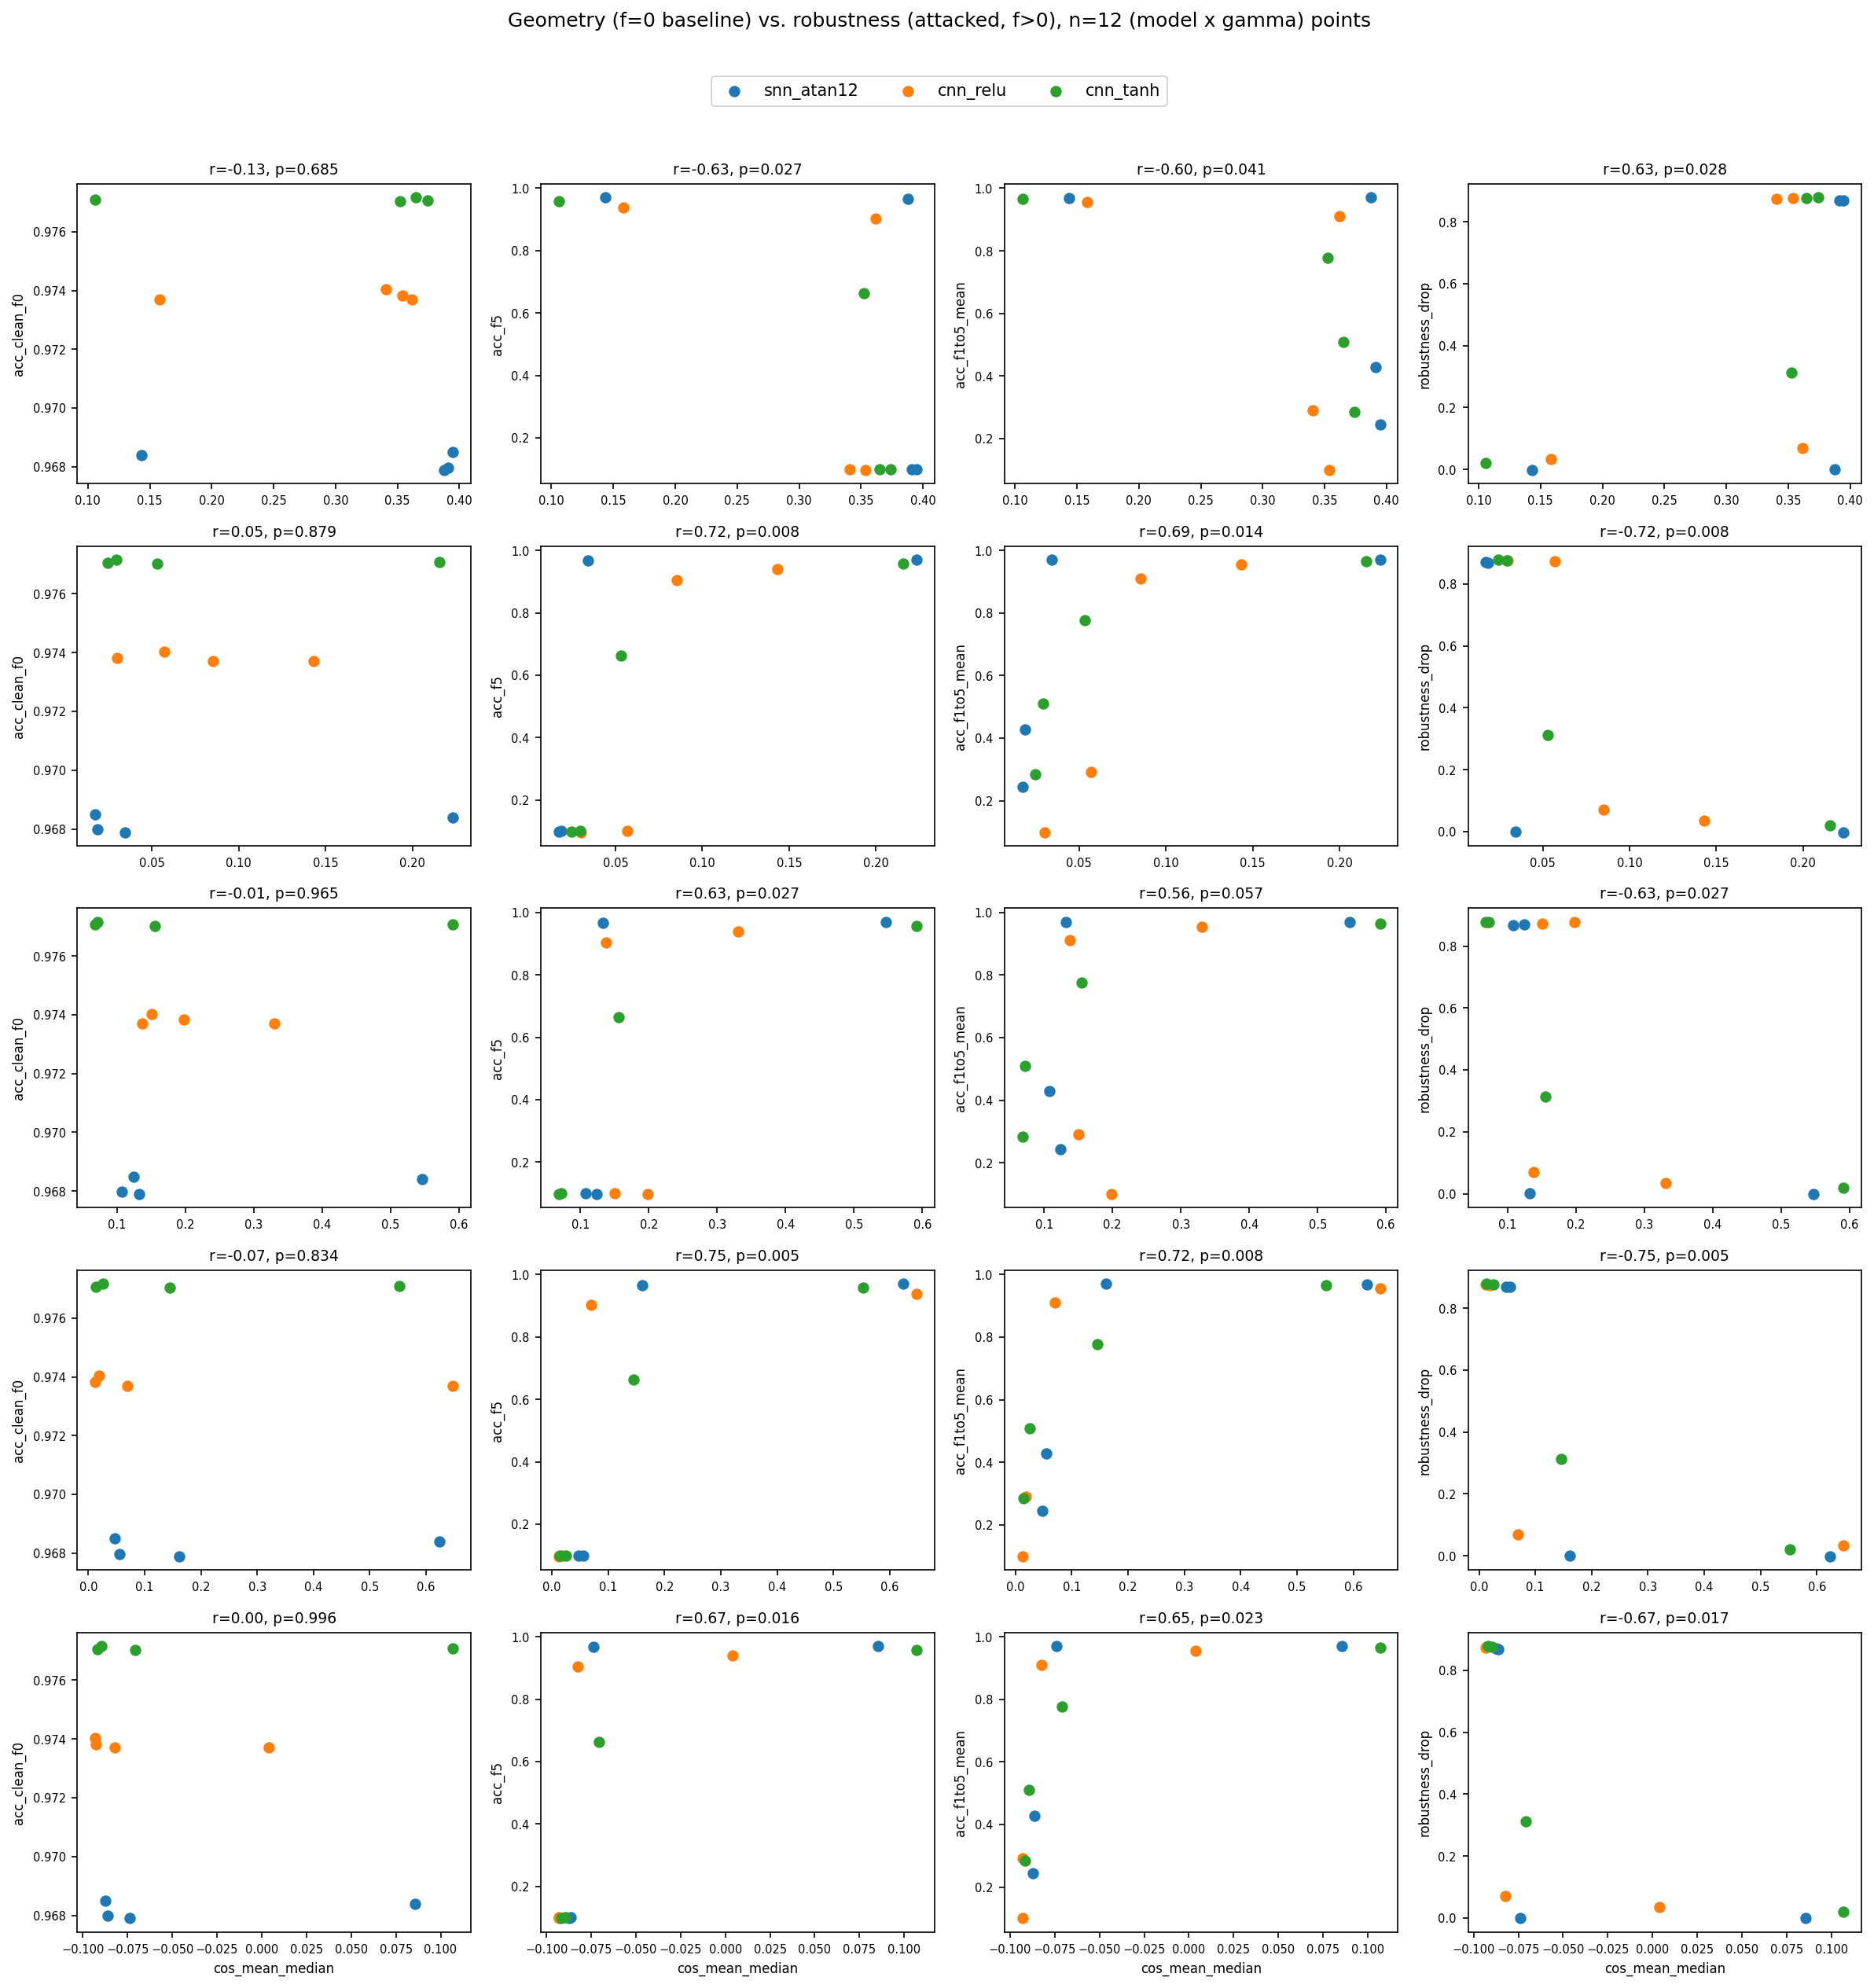
\includegraphics[width=\textwidth]{correlation_scatter.png}
    \caption{Each panel: one geometry metric (median, $f=0$, steps [100,400]) vs.\ one robustness summary, $n=12$ points (3 models $\times$ 4 $\gamma$). $r$ = Pearson correlation, $p$ = two-sided p-value.}
    \label{fig:correlation-scatter}
\end{figure}

\begin{center}
\small
\begin{tabular}{@{}llrrr@{}}
\toprule
Geometry metric & Robustness metric & $r$ & $p$ & $n$ \\
\midrule
$S_{\text{layer0}}$ & acc\_f5          & \phantom{-}0.751 & 0.005 & 12 \\
$S_{\text{layer0}}$ & robustness\_drop & $-0.750$          & 0.005 & 12 \\
$Q$                  & acc\_f5          & \phantom{-}0.725 & 0.008 & 12 \\
$S_{\text{layer0}}$ & acc\_f1to5\_mean & \phantom{-}0.724 & 0.008 & 12 \\
$Q$                  & robustness\_drop & $-0.724$          & 0.008 & 12 \\
$\cos_{\text{mean}}$ & acc\_f5          & \phantom{-}0.673 & 0.016 & 12 \\
$N$                  & acc\_f5          & $-0.633$          & 0.027 & 12 \\
$S$                  & acc\_f5          & \phantom{-}0.633 & 0.027 & 12 \\
\midrule
$N$                  & acc\_clean\_f0   & $-0.131$          & 0.685 & 12 \\
$S_{\text{layer0}}$ & acc\_clean\_f0   & $-0.068$          & 0.834 & 12 \\
$Q$                  & acc\_clean\_f0   & \phantom{-}0.049 & 0.879 & 12 \\
$S$                  & acc\_clean\_f0   & $-0.014$          & 0.965 & 12 \\
$\cos_{\text{mean}}$ & acc\_clean\_f0   & \phantom{-}0.001 & 0.996 & 12 \\
\bottomrule
\end{tabular}
\end{center}
Full table (20 metric pairs) in \texttt{correlation\_table.csv}. \texttt{acc\_f5} = worst-case accuracy at $f=5$; \texttt{acc\_f1to5\_mean} = mean worst-case accuracy over $f=1..5$; \texttt{robustness\_drop} = \texttt{acc\_clean\_f0} $-$ \texttt{acc\_f5}.

\textbf{Observed fact}: every geometry metric computed at $f=0$ correlates moderately-to-strongly ($|r|=0.63$ to $0.75$, $p<0.03$) with robustness metrics measured under attack ($f>0$) at the \emph{same} $\gamma$, across a 12-point sample (3 models $\times$ 4 $\gamma$). None of these same metrics correlates with clean, attack-free accuracy at $f=0$ ($|r|<0.14$, $p>0.68$ in all five cases).

\section{Interpretation}

The strongest, most consistent signal in this data is not a difference between architectures (SNN vs.\ ReLU vs.\ Tanh) but an almost universal effect of $\gamma$ (data heterogeneity) across all three: it drives $N$, $\cos_{\text{mean}}$'s sign flip, and the per-layer consensus redistribution seen in Section~4.1. The four originally registered predictions, which were architecture-centric, mostly failed outside the iid case ($\gamma=1.0$) -- so architecture differences in gradient geometry seem to be a $\gamma=1.0$-only phenomenon, not a general property of these models.

The correlation results are consistent with a specific, testable story: \emph{how much the honest clients agree with each other at $f=0$ (in sign, and directionally via cosine similarity) predicts how much slack the aggregator has left over to absorb Byzantine attackers, without predicting how well the model learns in the first place.} Concretely, $S$ and $Q$ (both consensus proxies) and $\cos_{\text{mean}}$ correlate positively with post-attack accuracy, while $N$ (dispersion) correlates negatively -- exactly the sign pattern one would expect if geometric agreement at $f=0$ is a leading indicator of the margin an aggregator like \texttt{TrMean}/\texttt{GeometricMedian} has before Byzantine votes can dominate a coordinate. The complete absence of correlation with clean accuracy ($f=0$, no attack) suggests these metrics are specifically informative about \emph{robustness headroom}, not general model quality -- which is the more useful (and non-trivial) property for this research question.

Two caveats limit how far this should be pushed. First, $n=12$ with 3 models $\times$ 4 $\gamma$ means these 12 points are not independent draws -- much of the correlation could be a $\gamma$-driven confound shared by both geometry and robustness, rather than geometry being causally informative beyond $\gamma$ alone; a partial-correlation or within-model check would be the natural next step. Second, the robustness numbers are a proxy (Section~\ref{sec:robustness-sources}): different aggregator (\texttt{GeometricMedian} instead of \texttt{TrMean}), different SNN $\alpha$ (1.25 vs.\ 1.2), different CNN~ReLU learning rate (0.05 vs.\ 0.15), and a single attack for the SNN row. The direction and rough size of the correlations are unlikely to be pure artifacts of these substitutions, but an exact-match sweep (same \texttt{TrMean}+\texttt{NNM}+\texttt{ARC}, same lr/$\alpha$, all 3 attacks, $f=0..5$) would be needed to confirm the effect sizes precisely.

\end{document}
